\subsection{Geodaten zu Hypotheken und Hochwasser}
\subsubsection{Hypothekengeodaten}
Für die Kompatibilität von Hypotheken- und Hochwasserdaten sind geografische Koordinaten erforderlich. Dieser Abschnitt befasst sich mit der Generierung präziser Koordinaten für die Datenpunkte.

Eine zufällige Verteilung in Bayern würde die Struktur eines Kreditportfolios nicht korrekt abbilden, da eine ungleichmäßige Verteilung von Immobilien sowohl in Deutschland als auch in Bayern zu beobachten ist. \textcite{zurek2022real} analysierte die Beziehung zwischen Bevölkerungsdichte und Kreditvergabe in Deutschland. Die Studie zeigt, dass Regionen mit stärkerem Wirtschaftswachstum höhere Immobilienpreise aufweisen. Dies führt zu einer erhöhten Kreditnachfrage. Auf Basis dieser empirischen Erkenntnisse wird die Bevölkerungsdichte als Grundlage für die Zuweisung spezifischer Koordinaten zu jedem Datenpunkt herangezogen.

Die verwendete Datenquelle stammt von \textcite{suche_postleitzahl}. Sie kombiniert OpenStreetMap-Daten mit Einwohnerzahlen von \textcite{destatis}. Dies ermöglicht eine präzise Segmentierung in Postleitzahlenzonen. Tabelle \ref{tab:geodaten} präsentiert die resultierenden Daten dieser räumlichen Strukturierung.

\begin{table}[htbp]
    \centering
    \small  % Adjust font size to make everything fit in the table
    \caption{Beschreibung der Geodaten in verschiedenen Postleitzahlgebieten in Bayern}
    \label{tab:geodaten}
    \begin{tabularx}{\textwidth}{lXcXcXc}
        \toprule
        \textbf{plz} & \textbf{einwohner} & \textbf{qkm} & \textbf{geometry} & \textbf{ort} & \textbf{landkreis} & \textbf{bundesland} \\
        \midrule
        81248 & 121  & 1984763  & POLYGON((…)) & München & & Bayern \\
        96103 & 8519 & 14585957   & POLYGON((…)) & Hallstadt & Landkreis Bamberg & Bayern \\
        63930 & 1552 & 16628516 & POLYGON((…)) & Neunkirchen & Landkreis Miltenberg & Bayern \\
        94530 & 2071 & 2414777 & POLYGON((…)) & Auerbach & Landkreis Deggendorf & Bayern \\
        85051 & 31592 & 3878506 & POLYGON((…)) & Ingolstadt & & Bayern \\
        63916 & 4002 & 51878059 & POLYGON((…)) & Amorbach & Landkreis Miltenberg & Bayern \\
        \dots & \dots & \dots & \dots & \dots & \dots & \dots \\
        83024 & 16249 & 9466746 & POLYGON((…)) & Rosenheim & & Bayern \\
        \bottomrule
    \end{tabularx}
\end{table}
Tabelle \ref{tab:geodaten} wurde aus Shapefile-Daten der Postleitzahlenregionen generiert und umfasst die Bevölkerungsverteilung. Vier Spalten sind von besonderer Relevanz: Ort, Landkreis, Geometrie und Einwohner. Die Geometriespalte enthält die geografischen Koordinaten der Gemeinden, dargestellt als Polygon oder Multipolygon. Ein Multipolygon setzt sich aus mehreren Einzelpolygonen verschiedener Formen zusammen. Zur räumlichen Referenzierung dient das Koordinatensystem EPSG:3035. Abbildung \ref{fig:bevoelkerungsdichte} visualisiert die aus diesen Daten abgeleitete Bevölkerungsdichteverteilung Bayerns nach Postleitzahlenbereichen.

\begin{figure}[htbp]
    \centering
    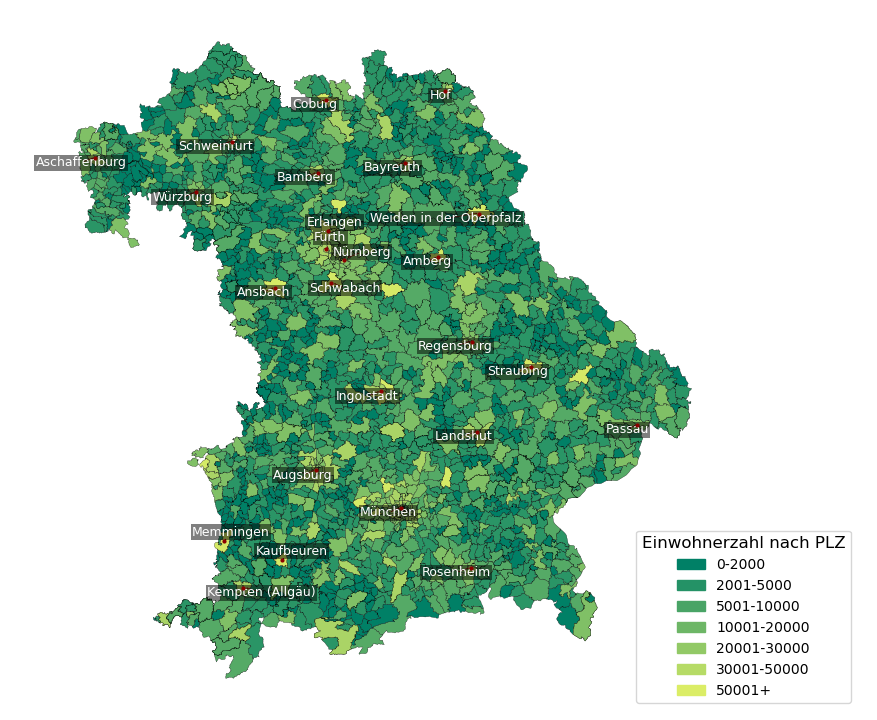
\includegraphics[width=0.95\textwidth]{figures/Bayern_pop_plz.png}
    \caption{Verteilung der Bevölkerungsdichte Bayerns nach Postleitzahlenbereichen}
    \label{fig:bevoelkerungsdichte}
\end{figure}
\clearpage

Zur repräsentativen Verteilung der 3853 Datenpunkte, die der Anzahl der Hypothekarkredite entsprechen, wird ein proportionaler Ansatz implementiert, der auf der Einwohnerzahl jeder Region basiert. Innerhalb der Postleitzahlgebiete erfolgt die Platzierung stochastisch. Es werden zufällige Koordinaten generiert und auf ihre Lage geprüft. Dieses Verfahren gewährleistet eine realitätsnahe räumliche Verteilung. Abbildung \ref{fig:hypothekenportfolio} zeigt die resultierende Distribution der Datenpunkte.



\begin{figure}[htbp]
    \centering
    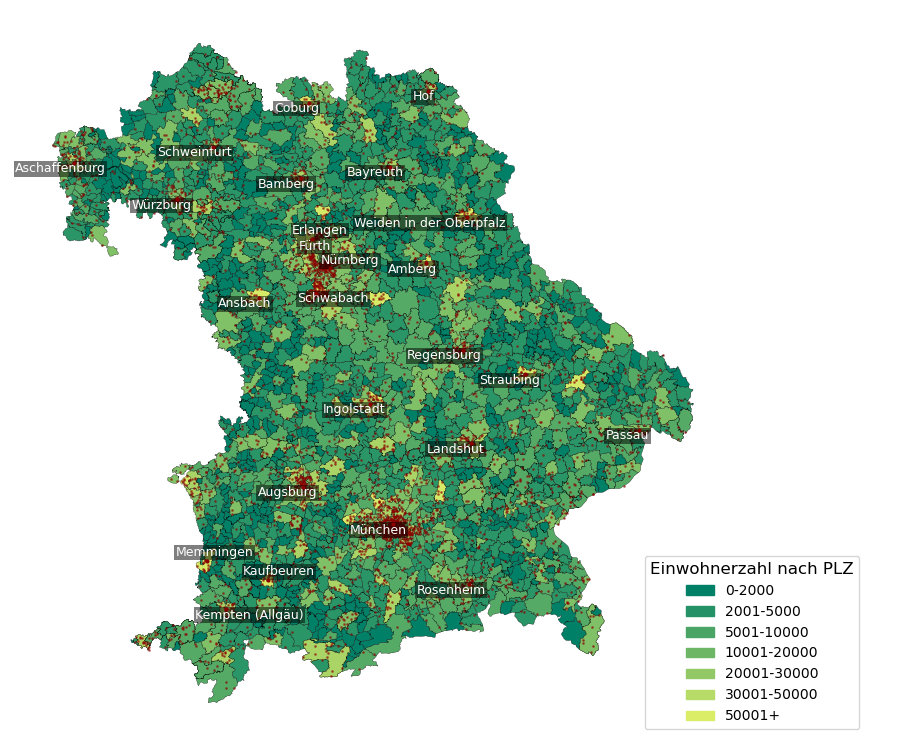
\includegraphics[width=\textwidth]{figures/bayern_por_pop.png} 
    \caption{Datenpunktverteilung im Hypothekenportfolio Bayern}
    \label{fig:hypothekenportfolio}
\end{figure}
\clearpage
\subsubsection{Hochwassergeodaten}